\documentclass[12pt,twoside]{report}


%use texdoc xxx to view the document about the package.

%chinese support.
\usepackage{xeCJK}
%mathtype support.
\usepackage{amsmath}
\usepackage{amsthm}
%page setting support.
\usepackage{geometry}
%figure insertion support.
\usepackage{graphicx}
%color support
\usepackage{xcolor}
%code block support
\usepackage{listings}
%drawing support
\usepackage{tikz}
%head foot set support
\usepackage{fancyhdr}
% 设置章节格式
\usepackage{titlesec} 
%font support
\usepackage{fontspec} 
%set indent
\usepackage{indentfirst}
%support box
\usepackage{framed}

\usepackage{caption}
\usepackage{algorithm}
\usepackage{algcompatible} 
\usepackage{algorithmicx} 
\usepackage{algpseudocode}
% \usepackage[linesnumbered,boxed]{algorithm2e}  

\usepackage[bookmarks=true,colorlinks,linkcolor=black]{hyperref}




%%%%%%%%%%%%%%%%%%%%%%%%%%%%%%%%%%%%%set color%%%%%%%%%%%%%%%%%%%%%%%%%%%%%%%%%%%%%%%%%%%%%%%%%%%%%%%
\definecolor{code-comments}{RGB}{0,180,0}   
\definecolor{background}{RGB}{234,244,244}

%%%%%%%%%%%%%%%%%%%%%%%%%%%%%%%%%%%%%set theoremstyle%%%%%%%%%%%%%%%%%%%%%%%%%%%%%%%%%%%%%%%%%%%%%%%%
\newtheoremstyle{nrush-thm-style}% hnamei
{20pt}% Space above
{20pt}% hSpace below
{\itshape}% Body font
{0pt}% Indent amount
{\bfseries\itshape\large}% Theorem head font
{:}% Punctuation after theorem head
{1em}% Space after theorem head
{}% Theorem head spec (can be left empty, meaning ‘normal’)

\theoremstyle{nrush-thm-style}

\makeatletter
\renewenvironment{proof}[1][Proof]{{\bfseries\large\itshape\noindent #1:\ \ }}{\ \rule{0.5em}{0.5em}}
\makeatother

%%%%%%%%%%%%%%%%%%%%%%%%%%%%%%%%%%%%%set pagesize%%%%%%%%%%%%%%%%%%%%%%%%%%%%%%%%%%%%%%%%%%%%%%%%%%%%
\geometry{a4paper,left=2cm,right=2cm,top=2cm,bottom=2cm}
\geometry{a4paper,vscale=0.9,hscale = 0.9}

%%%%%%%%%%%%%%%%%%%%%%%%%%%%%%%%%%%%%set foot%%%%%%%%%%%%%%%%%%%%%%%%%%%%%%%%%%%%%%%%%%%%%%%%%%%%%%%%
\pagestyle{plain}
\lhead{}
\chead{}
\rhead{}
\lfoot{}
\cfoot{}
\rfoot{\thepage}

%%%%%%%%%%%%%%%%%%%%%%%%%%%%%%%%%%%%%set paragraph-style%%%%%%%%%%%%%%%%%%%%%%%%%%%%%%%%%%%%%%%%%%%%%
% \setmainfont{Kozuka Mincho Pro R}
\setlength{\parindent}{2em}

%%%%%%%%%%%%%%%%%%%%%%%%%%%%%%%%%%%%%set code-style%%%%%%%%%%%%%%%%%%%%%%%%%%%%%%%%%%%%%%%%%%%%%%%%%%
\lstset{
backgroundcolor = \color{background},
keywordstyle=\color{blue!100},
commentstyle=\color{code-comments},
basicstyle=\small\sffamily ,
language=Matlab,
breaklines=true,
captionpos=b,
frame = single,
}

%%%%%%%%%%%%%%%%%%%%%%%%%%%%%%%%%%%%%set algorithm-style%%%%%%%%%%%%%%%%%%%%%%%%%%%%%%%%%%%%%%%%%%%%%%
\renewcommand{\algorithmicrequire}{\textbf{Input:}}  % Use Input in the format of Algorithm  
\renewcommand{\algorithmicensure}{\textbf{Output:}} % Use Output in the format of Algorithm

\makeatletter
\newenvironment{breakablealgorithm}
  {% \begin{breakablealgorithm}
   \begin{center}
     \refstepcounter{algorithm}% New algorithm
     \hrule height.8pt depth0pt \kern2pt% \@fs@pre for \@fs@ruled
     \renewcommand{\caption}[2][\relax]{% Make a new \caption
       {\raggedright\textbf{\ALG@name~\thealgorithm} ##2\par}%
       \ifx\relax##1\relax % #1 is \relax
         \addcontentsline{loa}{algorithm}{\protect\numberline{\thealgorithm}##2}%
       \else % #1 is not \relax
         \addcontentsline{loa}{algorithm}{\protect\numberline{\thealgorithm}##1}%
       \fi
       \kern2pt\hrule\kern2pt
     }
  }{% \end{breakablealgorithm}
     \kern2pt\hrule\relax% \@fs@post for \@fs@ruled
   \end{center}
  }
\makeatother


%%%%%%%%%%%%%%%%%%%%%%%%%%%%%%%%%%%%%set tikz%%%%%%%%%%$%%%%%%%%%%%%%%%%%%%%%%%%%%%%%%%%%%%%%%%%%%%%%%
\usetikzlibrary{calc,matrix,decorations.markings,decorations.pathreplacing}
\usetikzlibrary{arrows,shapes,chains}

% 设置中文日期格式
\renewcommand{\today}{\number\year 年 \number\month 月 \number\day 日}
% 设置中文目录
\renewcommand{\contentsname}{目 录}
% 设置章节格式
\titleformat{\chapter}{\raggedright\Huge\bfseries}{第\,\thechapter\,章}{1em}{}






\newtheorem{theorem}{Theorem}
\newtheorem{acknowledgement}[theorem]{Acknowledgement}
% \newtheorem{algorithm}[theorem]{Algorithm}
\newtheorem{axiom}{Axiom}
\newtheorem{case}[theorem]{Case}
\newtheorem{claim}[theorem]{Claim}
\newtheorem{conclusion}[theorem]{Conclusion}
\newtheorem{condition}[theorem]{Condition}
\newtheorem{conjecture}[theorem]{Conjecture}
\newtheorem{corollary}[theorem]{Corollary}
\newtheorem{criterion}[theorem]{Criterion}
\newtheorem{definition}[theorem]{Definition}
\newtheorem{example}[theorem]{Example}
\newtheorem{exercise}[theorem]{Exercise}
\newtheorem{lemma}[theorem]{Lemma}
\newtheorem{notation}[theorem]{Notation}
\newtheorem{problem}[theorem]{Problem}
\newtheorem{proposition}[theorem]{Proposition}
\newtheorem{remark}[theorem]{Remark}
\newtheorem{solution}[theorem]{Solution}
\newtheorem{summary}[theorem]{Summary}

\begin{document}
\title{\itshape{Shorthand Book}}
\author{Ji Youzhou}
\date{\today}
\maketitle
\thispagestyle{empty}
\newpage

\tableofcontents
\setcounter{page}{1}
\newpage

\chapter{ubuntu18.04}
\setcounter{page}{1}
\section{常用软件}
可以用apt命令安装的
\begin{leftbar}
    \begin{itemize}
        \item autotools : 自动生成makefile
        \item doxygen : 生成说明文档
        \item git : 代码管理工具
    \end{itemize}
\end{leftbar}

\section{git的使用}

\begin{leftbar}
    \begin{itemize}
        \item git init : 创建git库
        \item git add filename : 添加文件到缓冲区
        \item git commit -m "message" : 
        \item git diff filename :
        \item git status :
        \item git reset --hard HEAD s$\hat{}$ :
        \item git reset --hard v-id :
        \item git log :
        \item git log --graph :
        \item git reflog :
        \item git checkout -- filename :
        \item git reset HEAD filename :
        \item git rm filename :
        \item git remote add origin git@server-name:path/repo-name.git : 
        \item git push origin master : 
        \item git clone git@server-name:path/repo-name.git
        \item git checkout -b filename :
        \item git branch :
        \item git branch branch-name :
        \item git branch -d branch-name :
        \item gti branch -D branch-name :
        \item git checkout branch-name :
        \item git merge branch-name :
        \item git merge --no-ff -m "message" branch-name :
        \item git stash :
        \item git stash pop :
        \item git stash list :
        \item git stash apply :
        \item git stash apply stash@\{number\} :
        \item git stash drop :
        \item git stash drop stash@\{number\} :
        \item git branch --set-upstream-to <branch-name> origin/<branch-name> :
        \item git remote -v :
    \end{itemize}
\end{leftbar}


\section{安装texlive套件}
\begin{lstlisting}[language=sh]
    sudo apt install texlive-full
\end{lstlisting}

\section{vscode 支持 latex 编辑}
\begin{enumerate}
    \item 下载\textbf{LaTex WorkShop}扩展。
    \item 在\textbf{文件 $\rightarrow$ 首选项 $\rightarrow$ 设置 $\rightarrow$ LaTex $\rightarrow$ Chktex:Path} 中设置latex编译器路经,一般为\textbf{/usr/bin/}。
    \item 为支持中文,一般需要使用\textbf{XeLaTex}编译,这需要设置\textbf{文件 $\rightarrow$ 首选项 $\rightarrow$ 设置 $\rightarrow$ LaTex $\rightarrow$ Latex: Recipes},添加如下代码:
    \begin{lstlisting}[language=Java]
        "latex-workshop.latex.tools": [
            {
                "name": "latexmk",
                "command": "latexmk",
                "args": [
                    "-synctex=1",
                    "-interaction=nonstopmode",
                    "-file-line-error",
                    "-pdf",
                    "-outdir=%OUTDIR%",
                    "%DOC%"
                ],
                "env": {}
            },
            {
                "name": "pdflatex",
                "command": "pdflatex",
                "args": [
                    "-synctex=1",
                    "-interaction=nonstopmode",
                    "-file-line-error",
                    "%DOC%"
                ],
                "env": {}
            },
            {
                "name": "bibtex",
                "command": "bibtex",
                "args": [
                    "%DOCFILE%"
                ],
                "env": {}
            },
            {
                "name": "xelatex",
                "command": "xelatex",
                "args": [
                    "-synctex=1",
                    "-interaction=nonstopmode",
                    "-file-line-error",
                    "%DOC%"
                ],
                "env": {}
            }
        ],
        "latex-workshop.latex.recipes":[
            {
                "name": "xelatex",
                "tools": [
                    "xelatex"
                ]
            },
            {
                "name": "latexmk",
                "tools": [
                    "latexmk"
                ]
            },
            {
                "name": "pdflatex ➞ bibtex ➞ pdflatex × 2",
                "tools": [
                    "pdflatex",
                    "bibtex",
                    "pdflatex",
                    "pdflatex"
                ]
            }
        ], 
    \end{lstlisting}
\end{enumerate}

\section{换国内下载源}

\begin{enumerate}
    \item 备份文件。
    \begin{lstlisting}[language=sh]
        cp /etc/apt/sources.list /etc/apt/sources.list.bak
    \end{lstlisting}

    \item 添加新源。
    \begin{lstlisting}[language=sh]
vim /etc/apt/sources.list
#添加阿里源
deb http://mirrors.aliyun.com/ubuntu/ bionic main restricted universe multiverse
deb http://mirrors.aliyun.com/ubuntu/ bionic-security main restricted universe multiverse
deb http://mirrors.aliyun.com/ubuntu/ bionic-updates main restricted universe multiverse
deb http://mirrors.aliyun.com/ubuntu/ bionic-proposed main restricted universe multiverse
deb http://mirrors.aliyun.com/ubuntu/ bionic-backports main restricted universe multiverse
deb-src http://mirrors.aliyun.com/ubuntu/ bionic main restricted universe multiverse
deb-src http://mirrors.aliyun.com/ubuntu/ bionic-security main restricted universe multiverse
deb-src http://mirrors.aliyun.com/ubuntu/ bionic-updates main restricted universe multiverse
deb-src http://mirrors.aliyun.com/ubuntu/ bionic-proposed main restricted universe multiverse
deb-src http://mirrors.aliyun.com/ubuntu/ bionic-backports main restricted universe multiverse

##中科大源
deb https://mirrors.ustc.edu.cn/ubuntu/ bionic main restricted universe multiverse
deb-src https://mirrors.ustc.edu.cn/ubuntu/ bionic main restricted universe multiverse
deb https://mirrors.ustc.edu.cn/ubuntu/ bionic-updates main restricted universe multiverse
deb-src https://mirrors.ustc.edu.cn/ubuntu/ bionic-updates main restricted universe multiverse
deb https://mirrors.ustc.edu.cn/ubuntu/ bionic-backports main restricted universe multiverse
deb-src https://mirrors.ustc.edu.cn/ubuntu/ bionic-backports main restricted universe multiverse
deb https://mirrors.ustc.edu.cn/ubuntu/ bionic-security main restricted universe multiverse
deb-src https://mirrors.ustc.edu.cn/ubuntu/ bionic-security main restricted universe multiverse
deb https://mirrors.ustc.edu.cn/ubuntu/ bionic-proposed main restricted universe multiverse
deb-src https://mirrors.ustc.edu.cn/ubuntu/ bionic-proposed main restricted universe multiverse

##163源
deb http://mirrors.163.com/ubuntu/ bionic main restricted universe multiverse
deb http://mirrors.163.com/ubuntu/ bionic-security main restricted universe multiverse
deb http://mirrors.163.com/ubuntu/ bionic-updates main restricted universe multiverse
deb http://mirrors.163.com/ubuntu/ bionic-proposed main restricted universe multiverse
deb http://mirrors.163.com/ubuntu/ bionic-backports main restricted universe multiverse
deb-src http://mirrors.163.com/ubuntu/ bionic main restricted universe multiverse
deb-src http://mirrors.163.com/ubuntu/ bionic-security main restricted universe multiverse
deb-src http://mirrors.163.com/ubuntu/ bionic-updates main restricted universe multiverse
deb-src http://mirrors.163.com/ubuntu/ bionic-proposed main restricted universe multiverse
deb-src http://mirrors.163.com/ubuntu/ bionic-backports main restricted universe multiverse

##清华源
deb https://mirrors.tuna.tsinghua.edu.cn/ubuntu/ bionic main restricted universe multiverse
deb-src https://mirrors.tuna.tsinghua.edu.cn/ubuntu/ bionic main restricted universe multiverse
deb https://mirrors.tuna.tsinghua.edu.cn/ubuntu/ bionic-updates main restricted universe multiverse
deb-src https://mirrors.tuna.tsinghua.edu.cn/ubuntu/ bionic-updates main restricted universe multiverse
deb https://mirrors.tuna.tsinghua.edu.cn/ubuntu/ bionic-backports main restricted universe multiverse
deb-src https://mirrors.tuna.tsinghua.edu.cn/ubuntu/ bionic-backports main restricted universe multiverse
deb https://mirrors.tuna.tsinghua.edu.cn/ubuntu/ bionic-security main restricted universe multiverse
deb-src https://mirrors.tuna.tsinghua.edu.cn/ubuntu/ bionic-security main restricted universe multiverse
deb https://mirrors.tuna.tsinghua.edu.cn/ubuntu/ bionic-proposed main restricted universe multiverse
deb-src https://mirrors.tuna.tsinghua.edu.cn/ubuntu/ bionic-proposed main restricted universe multiverse
    \end{lstlisting}

    \item 更新。
    \begin{lstlisting}[language=sh]
        sudo apt update
        sudo apt upgrade
    \end{lstlisting}
\end{enumerate}

\section{python3 安装pip工具并升级}
\begin{lstlisting}[language=sh]
    #安装
    sudo apt install python3-pip
    #升级
    sudo pip3 install --upgrade pip
    #查看版本
    pip3 --version
\end{lstlisting}

\section{pip3 报错}
\noindent 错误提示:
\begin{lstlisting}[language=sh]
Traceback (most recent call last):
File "/usr/bin/pip3", line 9, in <module>
  from pip import main
ImportError: cannot import name 'main'  
\end{lstlisting}
解决方法:
\begin{lstlisting}[language=sh]
sudo gedit /usr/bin/pip3
sudo cp /usr/bin/pip3 /usr/bin/pip3.bak
\end{lstlisting}
将
\begin{lstlisting}[language=python]
from pip import main
if __name__ == '__main__':
    sys.exit(main())
\end{lstlisting}
替换为
\begin{lstlisting}[language=python]
from pip import __main__
if __name__ == '__main__':
    sys.exit(__main__._main())
\end{lstlisting}

\section{pip3 换国内源}
\begin{lstlisting}[language=sh]
mkdir ~/.pip
gedit ~/.pip/pip.conf
\end{lstlisting}

添加如下代码
\begin{lstlisting}[language=sh]
[global]
timeout = 6000
index-url = https://pypi.tuna.tsinghua.edu.cn/simple
trusted-host = pypi.tuna.tsinghua.edu.cn
\end{lstlisting}

\section{开启SSH服务}
\begin{lstlisting}[language=sh]
    #更新软件库信息
    sudo apt update
    #安装用户端
    sudo apt install openssh-client
    #安装服务端
    sudo apt install openssh-server
    #开启SSH服务
    sudo service ssh start
    #确认是否开启成功,ssh-agent表示client成功,sshd代表server成功。
    sudo ps -e|grep ssh
    #查看ip地址便于连接,这是局域网地址,公网ip地址在百度搜ip可以得到
    ifcofig
\end{lstlisting}

\chapter{C/C++}
\section{C++重载}
C++ 允许在同一作用域中的某个函数和运算符指定多个定义,分别称为函数重载和运算符重载。重载函数或符号的名称相同但其功能并不相同,编译器会根据使用的形式来确定是那一个操作。
运算符运算符重载格式
\begin{lstlisting}[language=C]
    <class-name> operator<operator-symbol>(inputs);
\end{lstlisting}
并非所有的运算符都可以重载,部分运算符如:
\begin{lstlisting}[language=C]
    .
    .*
    ->*
    ::
    ?:
    #
    sizeof
\end{lstlisting}
是不可以被重载的。

\chapter{Data structure}
\section{二叉树的前,中,候序遍历(DLR,LDR,LRD)的含义}
\begin{itemize}
    \item DLR: 根节点,左节点,右节点遍历。
    \item LDR: 左节点,根节点,右节点遍历。
    \item LRD: 左节点,右节点,根节点遍历。
\end{itemize}

\begin{figure}[H]
    \centering  
	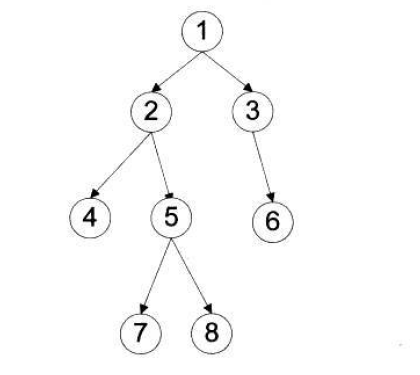
\includegraphics[width=0.3\linewidth]{pic/tree}  
	\caption{Tree}  
\end{figure}

\begin{itemize}
    \item DLR: 1 2 4 5 7 8 3 6
    \item LDR: 4 2 7 5 8 1 3 6
    \item LRD: 4 7 8 5 2 6 3 1
\end{itemize}

得到一颗树的LDR和DLR或LRD中的一种是可以获得唯一的树的,如果仅仅是DLR和LRD则无法唯一确定。

\chapter{Opencv}
\section{VS环境下鼠标移到Mat卡死问题}
Mat注释过长,转到Mat定义处(鼠标不停留选中),在Mat与注释间加一空行保存。

\section{分离RGB三通道}

\begin{lstlisting}[language=C]
    \\ 分配地址
    vector<Mat> bgr;
    \\ 分割窗口
    split(src,bgr); 
\end{lstlisting}

\section{图片显示过大问题}

\begin{lstlisting}[language=C]
    \\ 设置窗口可调整
    namedWindow("src", WINDOW_NORMAL); 
    \\ 调整窗口大小
    cvResizeWindow("src", 500, 500);
    imshow("src", src);   
\end{lstlisting}

\section{VS下,使用nameWindow函数,imshow时却出项两个同名窗口问题}

在\textbf{项目属性 $\rightarrow$ 链接器 $\rightarrow$ 输入 $\rightarrow$ 附加依赖项}中去掉两个\textbf{opencv\_worldxxx.lib}两个文件中的一个,debug时去掉不带d的。

\section{遍历Mat元数}
Mat::forEach()具有最高的效率,对于Mat::at和指针来说其实两者效率差不都,指针略优。

\chapter{杂项}

\section{半收敛算法}
所谓半收敛算法直观印象就是说,算法误差降低到某一低点后,又回升震荡,对判断何时真正停止算法照成了困扰。

\section{椭圆的通径与偏心率}
所谓通径,就是过焦点作垂直于长轴的直线,其与椭圆交于两点,这条线段的长度就叫做通径。偏心率指的是椭圆焦距与其长轴长度的比值。
\end{document}